\begin{enumerate}[label=\thechapter.\arabic*,ref=\thechapter.\theenumi]
\item Let y\brak{t}=x\brak{4t},where x\brak{t} is a continous-time periodic signal of $100$s.the fundamental period of y\brak{t} is (\textbf{rounded off to the nearest integer})
 \hfill(GATE IN 2023)\\
\solution
\item  A spring mass system is shown in the figure . Take the value of acceleration  due to gravity as $g=9.81m/s^2$.The static deflection due to weight and the time period of the oscillations,respectively,are\\\hfill{(GATE 2023 XE)}
 \begin{figure}[h!]
    \centering
    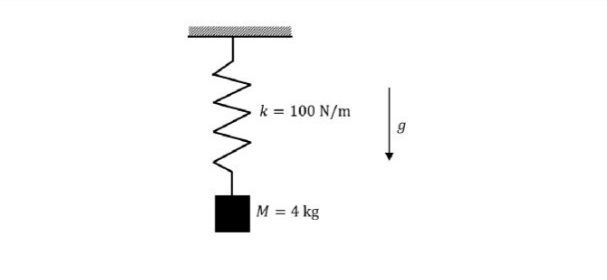
\includegraphics[width=0.4\textwidth]{2023/XE/71/figs/fig1.jpg}
\end{figure}
\solution
\end{enumerate}
